% MIRU2023 LaTeXクラスファイルの使い方 Ver.1
\documentclass[MIRU,submit,uplatex]{miru2023j}
\usepackage[dvipdfmx]{graphicx}
\usepackage{latexsym}
\usepackage[fleqn]{amsmath}
\usepackage[psamsfonts]{amssymb}
\DeclareMathOperator*{\argmax}{arg\,max} \DeclareMathOperator*{\argmin}{arg\,min}

\begin{document}

\title{順伝播型ニューラルネットワーク によるブラシスタイル変換}

\affiliate{Tokyo}{早稲田大学}
% \affiliate{Osaka}{第二大学(現在,第三コーポレーション勤務)}

 \author{木幡 咲希}{Saki KOHATA}{Tokyo}[cat-73@akane.waseda.jp]
 \author{シモセラ エドガー}{Edgar SIMO-SERRA}{Tokyo}[ess@waseda.jp]
%  \author{理解 次郎}{Jiro RIKAI}{Osaka}[jiro@rikai.co.jp]
%  \author{John Smith}{John Smith}{Osaka,Tokyo}[john@rikai.co.jp]

\maketitle

\section*{概要}
機械学習の発達により, 絵を描く技術の有無にかかわらず, 多くの人が完成度の
高い絵を生成できるようになった.しかし, 機械学習を用いた絵の生成に取り組む
研究のほとんどは画像をアーティスティックなスタイルに変更したり, テキスト
をもとに画像を生成したりなど, 既にクリエイターとして働いている人が使える
ツールであるとは言い難い. 本研究では, 人間が描いた絵のブラシスタイルを最適化に
よって推定し, 新たな入力画像をその推定したブラシスタイルを用いて再描画した画像を生成
するモデルを提案する. これにより, クリエイターの絵の制作プロセスを大幅に
効率化できることが期待される.
 

\section{序論}
人間は, 絵画を通じて自分の感情や思考を表現することに価値を見出してきた.
優れた作品を生み出すためには, 構図やスケッチ技術, 色彩や照明効果などを学ぶ必要が
あり, その習得には長い時間がかかるものであった. しかし, AI技術の進歩により, 
絵を描く技術のない人にも完成度の高い絵画を生成することが可能となった.
例えば, Midjourney\cite{Midjourney}は, 描いてほしい絵のイメージを単語や文章, キーワード
で入力するだけで素晴らしい絵画を生成することができるソフトウェアである. 
Midjourneyは, 使い方が簡単であることや生成された絵画が高品質であることから
人気であり, クリエイターにも高く評価されている.
しかし, このようなツールは, すでに自分のスタイルを確立したクリエイターにとって
役に立つツールであるとは言い難い. 
クリエイターにとっては, デジタル・アナログを問わず, 自分の手で作品を作ることが
重要であり, Midjourneyのように絵の生成課程の全てがAI技術に頼ったツールでは, 
描かれたオブジェクトの形状や色合いなどに不満が残ると考えられるからである.
私たちは, クリエイターが作業の途中に使えるような, 
クリエイターの支援につながる研究を行いたいと考えた.
そこで, クリエイターが描いた絵のブラシスタイルを推定し, そのブラシスタイルを
新たな画像に適応するモデルを開発することを目標とした.

本研究で提案したいモデルは, コンテンツ参照画像とスタイル参照画像の
2つの画像を入力とし, コンテンツ参照画像に描かれたものをスタイル参照画像の
ブラシスタイルで再描画した画像を生成するモデルである. 
図\ref{fig:haru}に, 2つの入力画像と出力画像の例を示す.
コンテンツ参照画像に示す絵はべた塗り用のブラシで作成したものであるため, 色と色の
境界線が常にはっきりしている. スタイル参照画像に示す絵は, アナログの絵のような
質感のブラシを使用して作成したものであるため, 色と色の境界線をグラデーションに
することも可能である.
生成画像はコンテンツ参照画像に描かれたものをスタイル参照画像のブラシスタイルで
表現したものとなっている. 図\ref{fig:haru}に示すコンテンツ参照画像のような画像を簡単な
ブラシを用いて手動で作成し,それをモデルに入力してクリエイターのブラシスタイルで
再描画させることで, クリエイターが絵の制作プロセスを大幅に効率化できることが期待
される. コンテンツ参照画像はクリエイターが作成するものであるため, オブジェクトの
形や色はクリエイターがコントロールすることができ,生成画像に対する不満は多少の修正
によって解消できると考えられる.
\begin{figure}
    \centering
    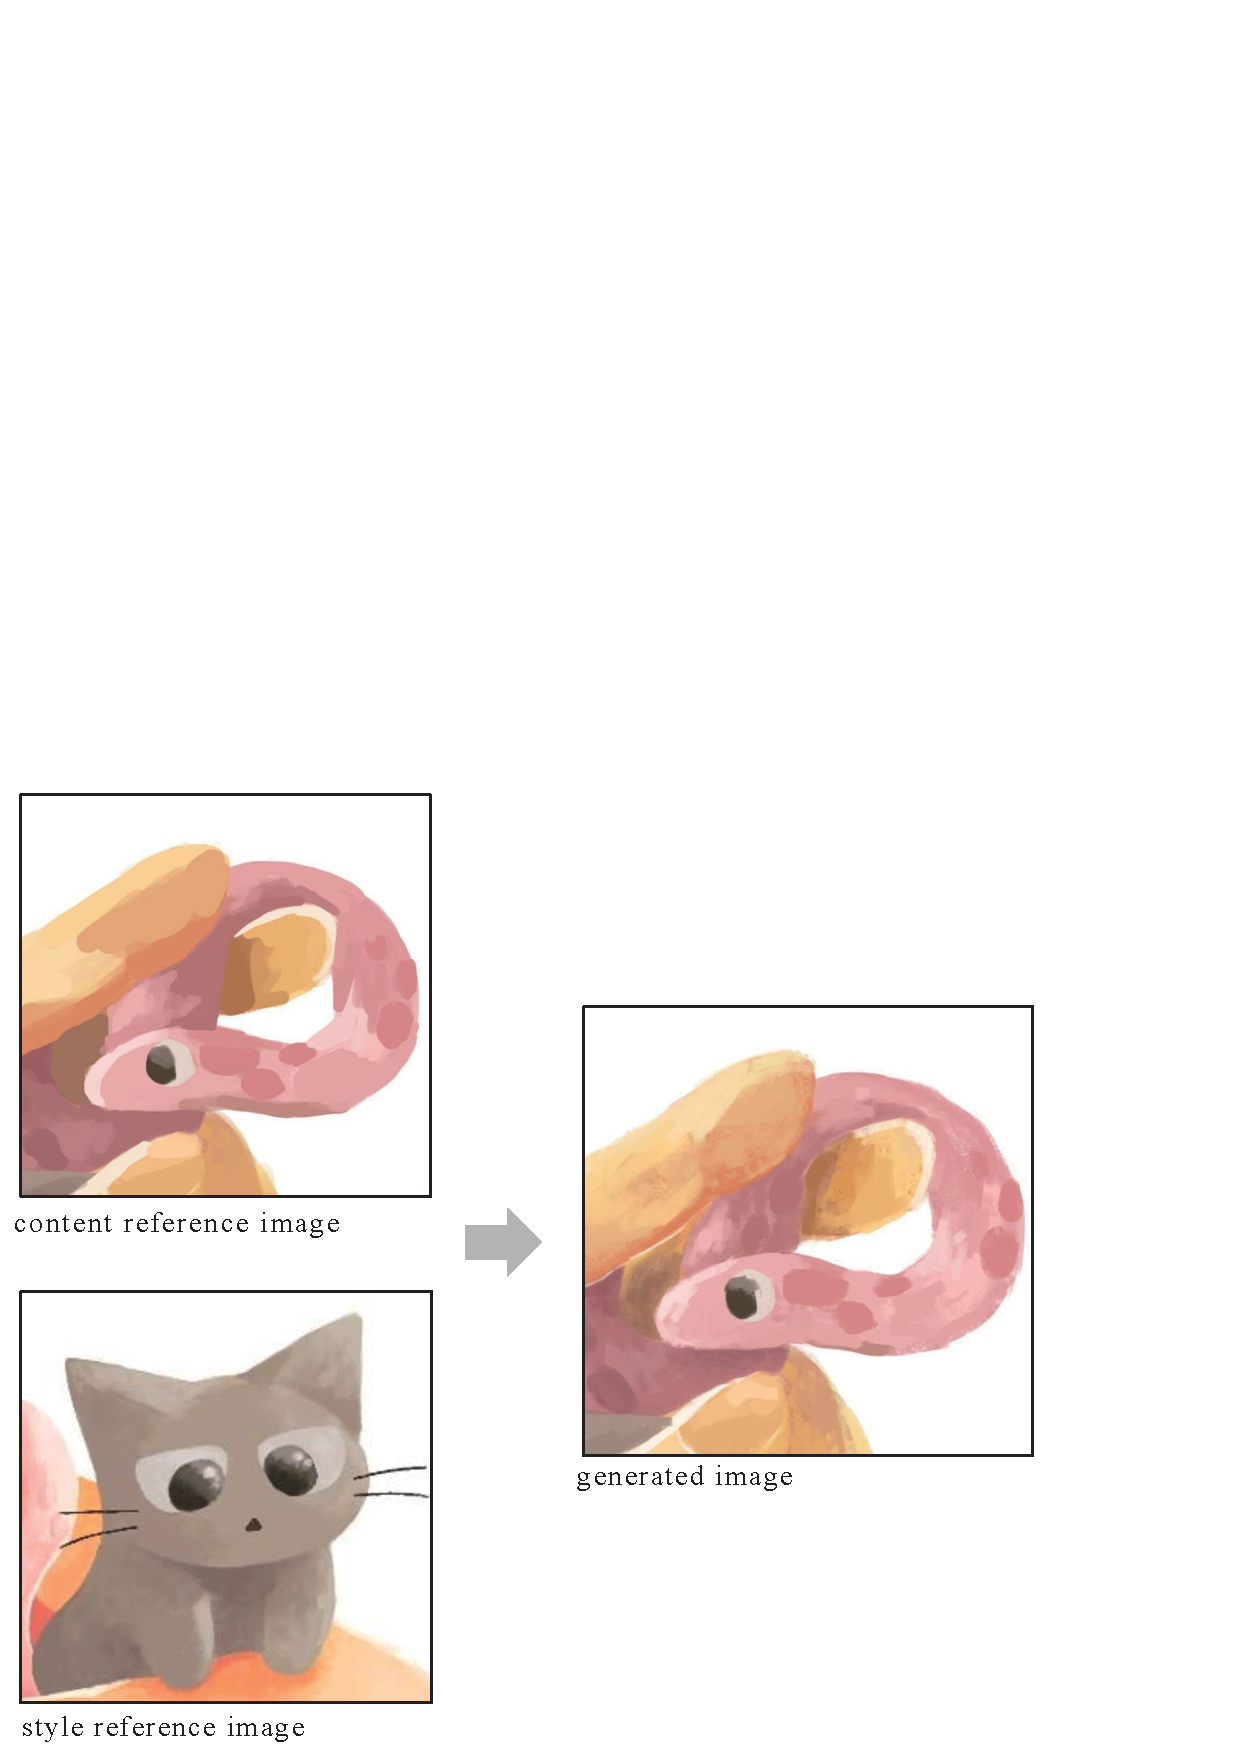
\includegraphics[width=1.0\linewidth]{resource/haru.pdf}
    \caption{作成したいモデルの入力画像と出力画像の例.}
    \label{fig:haru}
\end{figure}

\begin{figure*}[t]
    \centering
    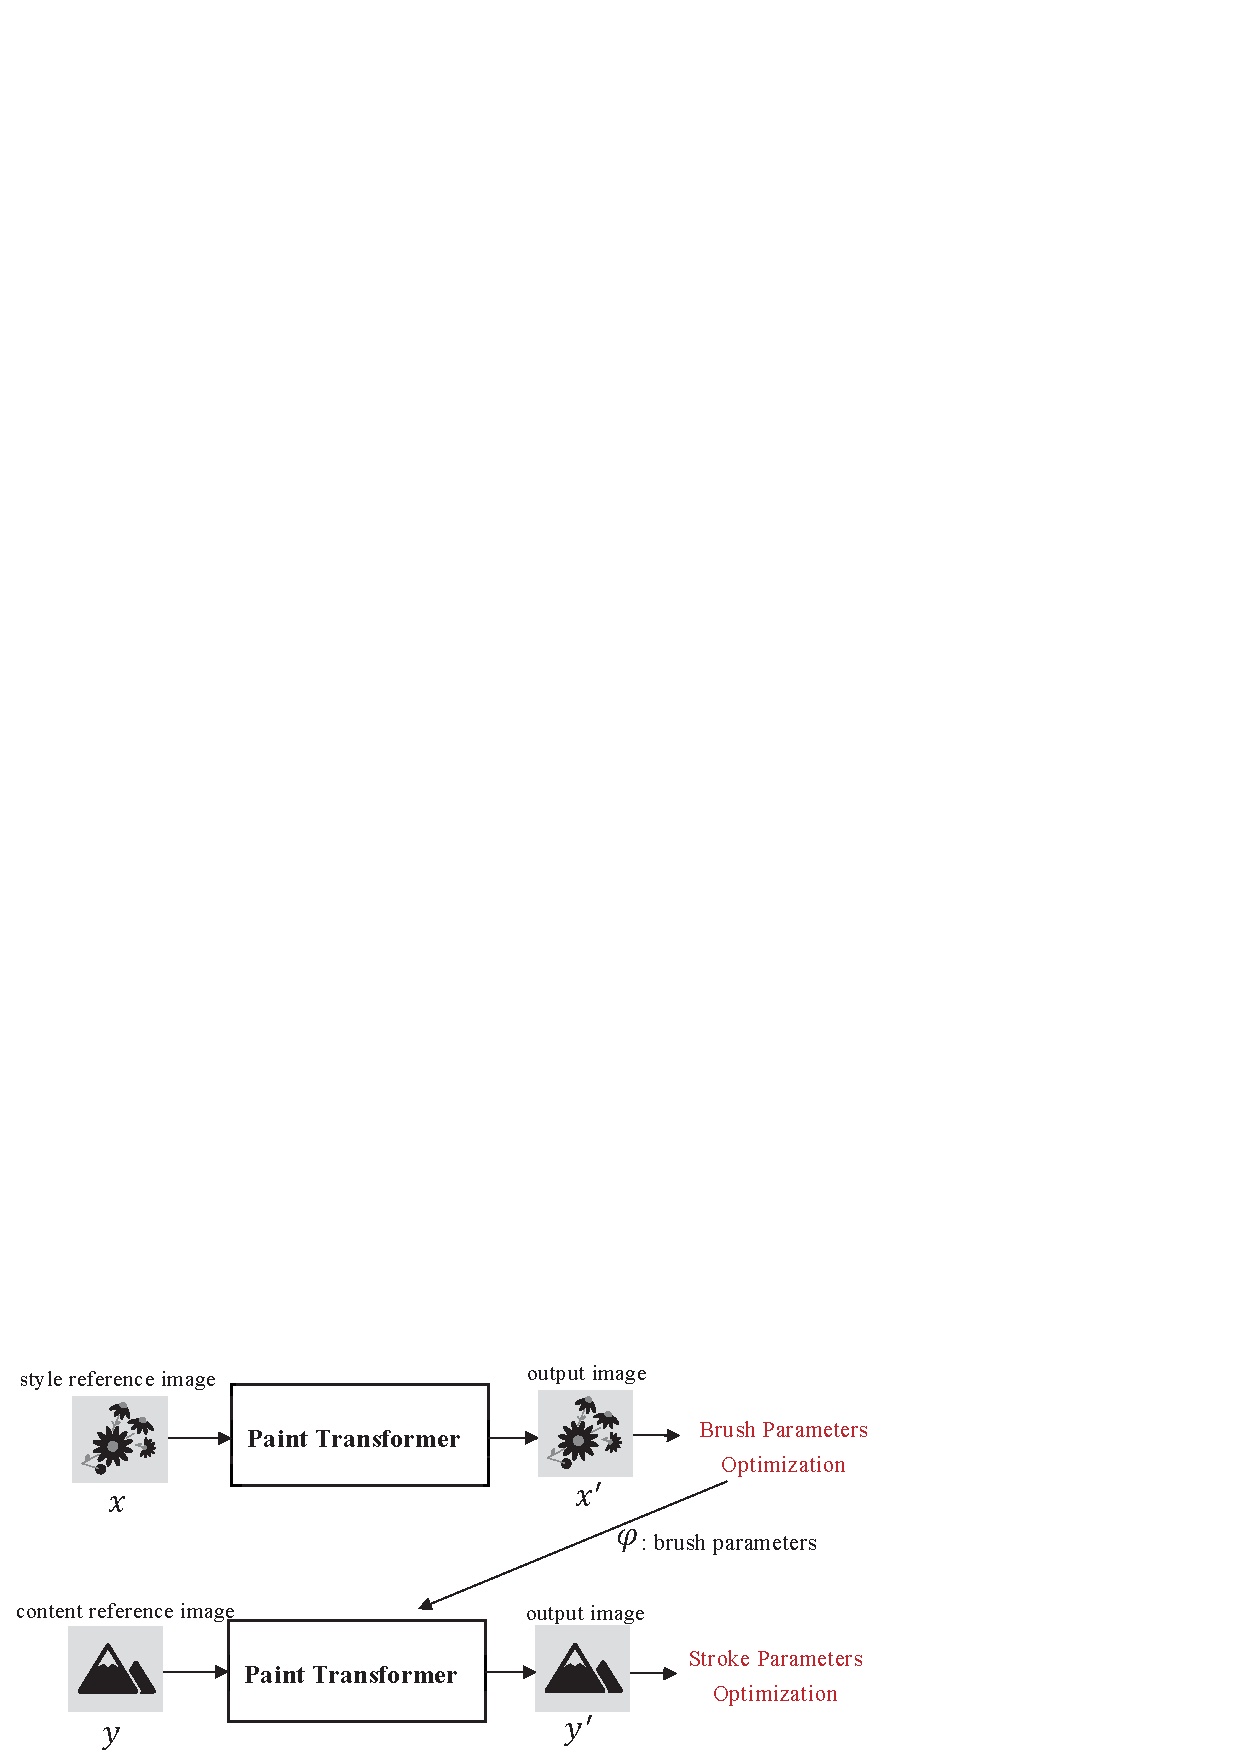
\includegraphics[width=0.9\linewidth]{resource/target_model.pdf}
    \caption{提案モデルのアーキテクチャの概要. 
    まず, 最適化を通じてスタイル画像からブラシパラメータ $s^g$ を推定し, 
    推定したブラシパラメータを用いてコンテンツ画像を再描画する. 
    }
    \label{fig:final_model}
\end{figure*}

\section{関連研究}
機械学習を用いた画像生成は盛んに研究されており, 大きな進歩を遂げている. 生成ツールとして
ニューラルネットワークを用いる手法は, 一般的にピクセル単位のマッピング\cite{PerceptualLosses}
やピクセル空間での連続的な最適化処理\cite{IST}として定式化されている.
しかし, 人間が絵を描くプロセスをニューラルネットワークが模倣することは困難である. 人間は絵を描く際,
まず大まかな色を塗ってから徐々に細部の描画に進んでいく方法が一般的だが, ニューラルネットワーク
はピクセルごとに画像を生成する. 人間の描画プロセスを模倣するためには, 機械は与えられた画像を順序付けられた
ストローク列に分解できなければならない. ニューラルネットワークは少ないストローク数でスケッチ
\cite{DBLP:journals/corr/HaE17}, \cite{DBLP:journals/corr/abs-1805-00247}, 落書き
\cite{DBLP:journals/corr/abs-1810-05977} を生成できるが, 特徴的なブラシスタイルで描かれた
イラストを生成するにはより多くのストロークが必要である. ストロークの全てに損失関数の設定を行い, 
ストロークの正解データを用意することは困難である. そのため, そのような画像のストローク分解を
行う際には, 強化学習がよく使われる. \cite{DBLP:journals/corr/abs-1804-01118, DBLP:journals/corr/abs-1206-4634, Huang_2019_ICCV}
強化学習エージェントの学習は計算コストが高いため, これをストロークパラメータ探索として定式化した研究も存在する. 
\cite{PaintTransformer}
本論文で扱うブラシのスタイル変換は, 絵画などの入力画像の全体的な雰囲気をCNNを用いて別の画像に転送
するNeural Style Transfer\cite{IST}で扱っているものと似ている. 論文内で提案されたモデルは
風景写真を芸術的なスタイルに変換することができるが, スタイル参照画像の全体的な雰囲気や色がコンテンツ参照
画像に反映されている. そのため, スタイル参照画像には描かれているがコンテンツ参照画像には存在しない
オブジェクトが, モデルからの出力画像に現れてしまう.
本研究では, コンテンツ参照画像に描かれた内容や色は変えずに,
ブラシのスタイルだけを転送することを目的としている. この問題にとりかかるにあたり, 
Liuら\cite{PaintTransformer}が提案したTransformerをベースとしたストローク生成パイプラインを,
提案モデルのストローク予測モデルとして採用した.

\section{提案手法}
提案手法の概要を図\ref{fig:final_model}に示す. 
まず, スタイル画像 $I_{style}$ を表現するストロークパラメータ $S_l$ と
ブラシスタイル $\hat{s}_g$ をみつける. 次に, ブラシスタイル $\hat{s}_g$ を固定し, 
スタイル参照画像のブラシスタイルで描かれたコンテンツ画像を表現するためのストローク
パラメータ $S_l'$ をみつける. 
ここで, ストロークパラメータはストロークの色や大きさのような, ストロークごとに
異なるパラメータのことを指し, ブラシパラメータはベースとなるブラシ画像などの, 
すべてのストロークに共通するパラメータを指す. 

\subsection{フレームワーク}
提案手法は, ストロークパラメータ $S_l$ とブラシスタイル $s_g$ から画像を再描画
することができるストローク予測モデル $M$ を中心に構成されている. 
まず, ストローク予測モデル $M$ の出力とスタイル参照画像 $I_{style}$ との
ストローク誤差を測定する損失関数 $L$ を最小化することによってブラシスタイル
$\hat{s}_g$ を定める: 
\begin{equation}
    \hat{s}_g = \argmin_{s_g} \;
        \min_{S_l} \;
           L\left( M\left(S_l, s_g\right), I_{style}\right)
    \label{eq_first}
\end{equation}
次に, ブラシスタイル $\hat{s}_g$ を固定し, 再びストローク誤差の最小化を行うが,
今度はコンテンツ参照画像 $I_{content}$ を対象とする: 
\begin{equation}
    \hat{S}_l = \argmin_{S_l} (L(M(S_l, \hat{s}_g), I_{content}))
    \label{eq_second}
\end{equation}
最終的な出力画像は, ストローク予測モデルを用いて, $S_l$ で表される最適なストロークと
$\hat{s}_g$ で表される最適なブラシスタイルによって計算される.
\begin{equation}
    I_{output} = M( \hat{S}_l, \hat{s}_g )
\end{equation}

\begin{figure}
    \centering
    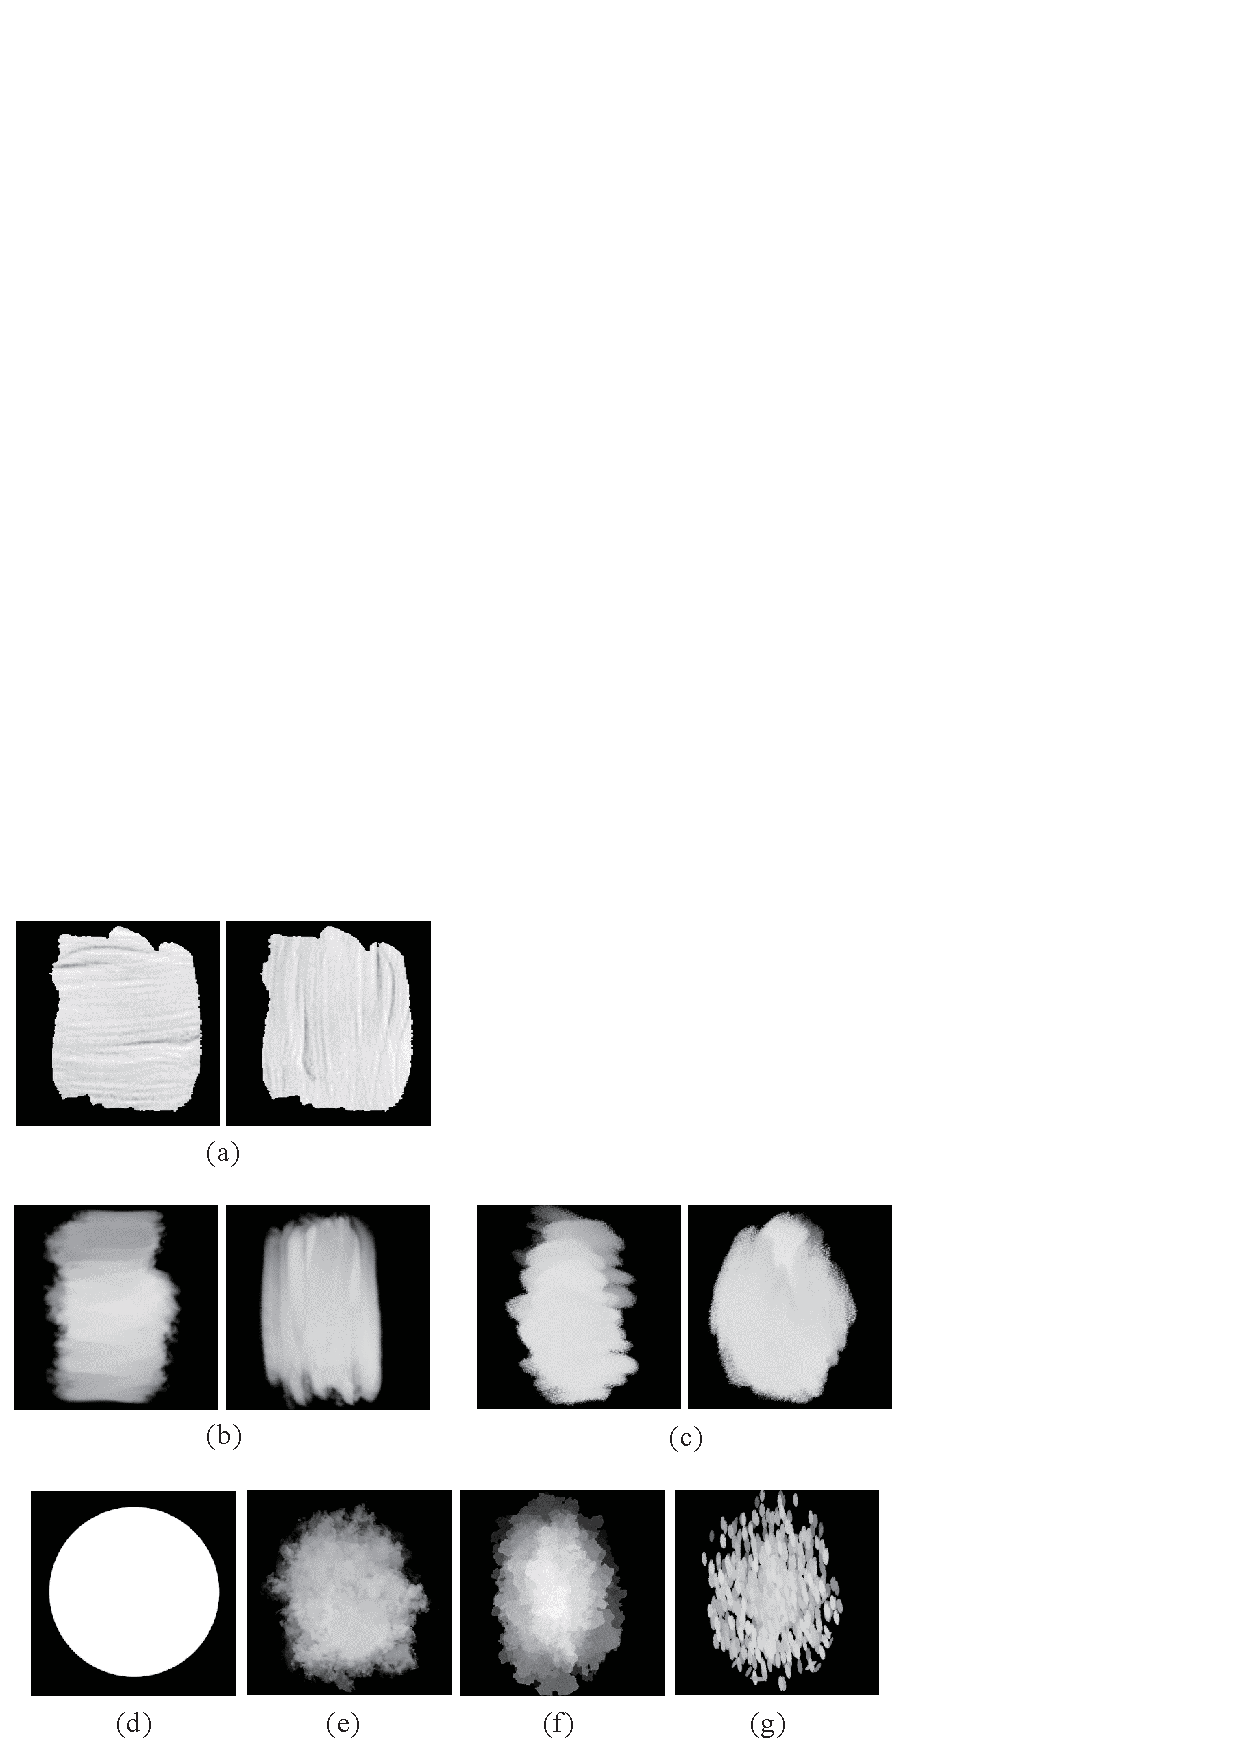
\includegraphics[width=1.0\linewidth]{resource/brushes.pdf}
    \caption{スタイル参照画像のブラシスタイルを正確に模倣するために作成した複数のブラシ画像.}
    \label{fig:brushes}
\end{figure}
 
\subsection{ストローク予測モデル}
ストローク予測モデル $M$ として, Liuら\cite{PaintTransformer}が提案したPaint Transformer
というTransformerベースのフレームワークを利用した. Paint Transformerは順伝播型変換器
を用いてストローク列を生成するTransformerベースのフレームワークである.
Paint Transformerは, ストローク予測器とストロークレンダラーの2つのモジュールから構成
される. ストロークは, 中心座標 $x$, $y$, 高さ $h$, 幅 $w$, 回転角 $\theta$, そして
色を表すRGBにそれぞれ対応する $r$, $g$, $b$ の8つのパラメータから成る. 
よって, 各ストローク $s$ は$s = \{ x, y, h, w, \theta, r, g, b \}$ と表すことができる.
Paint Transformerによってレンダリングされるストロークは, ベースとなるブラシ画像に拡大縮小
と回転をほどこし, 色を与えた単色のストロークである. Paint Transformerは, ランダムに
生成された8つのパラメータから複数のストロークを生成し, それらを訓練データとして使用して
ストローク予測器をトレーニングする. つまり, 訓練データはランダムに自動生成されるため,
データセットを用意する必要がない.

\subsection{ブラシスタイル}
Paint Transformerでは, 1種類のブラシ画像をベースとしてストロークを生成していた.
私たちは今回新たに6種類のブラシ画像を作成した. 図\ref{fig:brushes}に7種類のブラシ
画像を示す. (a)はLiuらが使用したブラシ画像であり, (b)~(g)が新たに作成したもの
である. (a)~(c)は水平方向のストロークと垂直方向のストロークのそれぞれに
ブラシ画像が用意されている. 


\begin{figure}
    \centering
    \includegraphics[width=1.0\linewidth]{resource/inputimg.pdf}
    \caption{実験に用いたコンテンツ参照画像(上段)とスタイル参照画像(下段).}
    \label{fig:inputs}
\end{figure}

\begin{figure*}[t]
    \centering
    \includegraphics[width=0.65\linewidth, angle=90]{resource/result.pdf}
    \caption{(a)モデルに入力したスタイル参照画像と提案モデルからの出力画像.
    (b)Neural Style Transferによる実行結果.}
    \label{fig:result}
\end{figure*}

\section{実験と結果}

\subsection{実験}
提案モデルはコンテンツ参照画像とスタイル参照画像を取り込み, 結果画像を出力する.
使用したコンテンツ参照画像とスタイル参照画像を図\ref{fig:inputs}に示す.
上段2枚がコンテンツ参照画像であり, 下段3枚がスタイル参照である.
コンテンツ参照画像はべた塗りのブラシ, スタイル参照画像は様々な特徴のあるブラシで
描いたものを用いた.

\subsection{結果}
図\ref{fig:brushes}に示した7種のブラシ画像を用いて図\ref{fig:inputs}の
コンテンツ参照画像を表現するストロークを生成した際に, 図\ref{fig:inputs}の
スタイル参照画像との類似度が最も高いとされた画像は図\ref{fig:result}の(a)に示す通りに
なった. 図\ref{fig:result}は, 各スタイル参照画像の横に並ぶ画像が, 
そのスタイル参照画像に最も類似したスタイルでコンテンツ参照画像を描いた結果であることを
意味するが, ブラシスタイルが模倣されているとは言い難い結果になっていることがわかる. 
これは, ベースとなるブラシ画像が7つのみであったことと, ストロークを表現するための
パラメータが最小限であることに起因していると考えられる.
出力画像に描かれた内容については, コンテンツ参照画像のものから大きく変化していない
ことが確認できる.
図\ref{fig:result}の(b)は, コンテンツ参照画像をNeural Style transfer(NST) \cite{IST}
に入力した際に得られる出力画像である. ブラシのスタイルは提案モデルに比べて高い精度で
模倣されているが,元のコンテンツ参照画像から色が変わっていたり, 
スタイル参照画像に描かれているオブジェクトが出現していたりすることがわかる.


\section{考察}
本研究では, 順伝播型ニューラルネットワークを利用して, コンテンツ参照画像の内容を
スタイル参照画像のブラシスタイルを模倣したスタイルに変換する新しいアプローチを
提案した. 私たちは, コンテンツ参照画像に描かれた内容をスタイル参照画像のブラシスタイルを
用いて再描画するために, Paint Transformer \cite{PaintTransformer} という
Transformerベースのフレームワークを利用した. 
提案モデルでは, Paint Transformerをそのまま使用してストローク予測モデルを
学習させたため, ストロークパラメータの種類もPaint Transformerと同様であり,  
5つの形状パラメータと3つの色パラメータの合計8つであった. 
今後の研究では, より多くのパラメータを追加することによって, より柔軟なブラシ
ストローク表現が可能になると考えられる. 提案モデルで生成されるストロークは, 
図\ref{fig:brushes}に示したブラシ画像を拡大・縮小・回転することによって作成
されているが, ストロークはブラシ画像を連続して複数繋げるという方法で
生成することも可能である. 
例えば, ペイントソフトのCLIP STUDIO PAINT\cite{ClipStudio}では, 図\ref{fig:discussion}
の右上に示すようなストロークを描くことができるが, 単にブラシ画像の大きさを調整する
だけでは同様のストロークを生成することはできず, 図\ref{fig:discussion}の右下の
ようなストロークとなってしまう. 
ストロークパラメータの種類を増やすことによってブラシの表現力を高め, 
図\ref{fig:discussion}の右上のようなストロークを生成できるようにすることで, 
スタイル参照画像のブラシスタイルを模倣した画像を生成可能になることが期待される. 
\begin{figure}[t]
    \centering
    
\includegraphics[width=1.0\linewidth]{resource/brush_discussion.pdf}
    \caption{提案モデルで使用したブラシの画像(左)と
    ClipStudioを用いて描いたストローク(右下)と
    ClipStudioで描いたストロークにあわせてブラシ画像を引き延ばしたもの(右上).}
    \label{fig:discussion}
\end{figure}
%\input{example_paper_text_jp.tex}

\newpage
\bibliographystyle{miru2022j}
\bibliography{myref}

\begin{thebibliography}{10}% 文献数が10未満の時 {9}
\bibitem{Midjourney}
“Midjourney,” Accessed: 2023-01-09. [Online]. Available: https://midjourney.com/.

\bibitem{PerceptualLosses}\sloppy
J. Johnson, A. Alahi, and L. Fei-Fei, “Perceptual losses for real-time
style transfer and super-resolution,” \textit{CoRR}, vol. abs/1603.08155, 2016.
arXiv: 1603 . 08155. [Online]. Available: http://arxiv.org/abs/1603.08155.

\bibitem{IST}
L. A. Gatys, A. S. Ecker, and M. Bethge, “Image style transfer using
convolutional neural networks,” in Proceedings of the IEEE Conference
on Computer Vision and Pattern Recognition (CVPR), Jun. 2016.

\bibitem{DBLP:journals/corr/HaE17}\sloppy
D. Ha and D. Eck, “A neural representation of sketch drawings,” \textit{CoRR},
vol. abs/1704.03477, 2017. arXiv: 1704 . 03477. [Online]. Available:
http://arxiv.org/abs/1704.03477.

\bibitem{DBLP:journals/corr/abs-1805-00247}
J. Song, K. Pang, Y. Song, T. Xiang, and T. M. Hospedales, “Learning
to sketch with shortcut cycle consistency,” \textit{CoRR}, vol. abs/1805.00247,
2018. arXiv: 1805.00247. [Online]. Available: http://arxiv.org/abs/
1805.00247.

\bibitem{DBLP:journals/corr/abs-1810-05977}
T. Zhou, C. Fang, Z. Wang, J. Yang, B. Kim, Z. Chen, J. Brandt,
and D. Terzopoulos, “Learning to sketch with deep q networks and
demonstrated strokes,” \textit{CoRR}, vol. abs/1810.05977, 2018. arXiv: 1810.
05977. [Online]. Available: http://arxiv.org/abs/1810.05977.

\bibitem{DBLP:journals/corr/abs-1804-01118}
Y. Ganin, T. Kulkarni, I. Babuschkin, S. M. A. Eslami, and O. Vinyals,
“Synthesizing programs for images using reinforced adversarial learn
ing,” \textit{CoRR}, vol. abs/1804.01118, 2018. arXiv: 1804.01118. [Online].
Available: http://arxiv.org/abs/1804.01118.

\bibitem{DBLP:journals/corr/abs-1206-4634}
N. Xie, H. Hachiya, and M. Sugiyama, “Artist agent: A reinforcement
learning approach to automatic stroke generation in oriental ink paint
ing,” \textit{CoRR}, vol. abs/1206.4634, 2012. arXiv: 1206 . 4634. [Online].
Available: http://arxiv.org/abs/1206.4634.

\bibitem{Huang_2019_ICCV}
Z. Huang, W. Heng, and S. Zhou, “Learning to paint with model-based
deep reinforcement learning,” in \textit{Proceedings of the IEEE/CVF Inter
national Conference on Computer Vision (ICCV)}, Oct. 2019.

\bibitem{PaintTransformer}
S. Liu, T. Lin, D. He, F. Li, R. Deng, X. Li, E. Ding, and H. Wang,
“Paint transformer: Feed forward neural painting with stroke prediction,”
in Proceedings of the IEEE International Conference on Computer Vision, 2021.

\bibitem{ClipStudio}
“CLIP STUDIO PAINT,” Accessed: 2023-01-09. [Online]. Available: https://www.clipstudio.net/.


\end{thebibliography}

\end{document}
